%نام و نام خانوادگی:
%شماره دانشجویی: 
\مسئله{پارسر \lr{LR(1)}}
\پاسخ{ }
\\
الف) عکس دیاگرام در زیر قرار داده شده است:
\graphicspath{{./images/}}
\begin{center}
	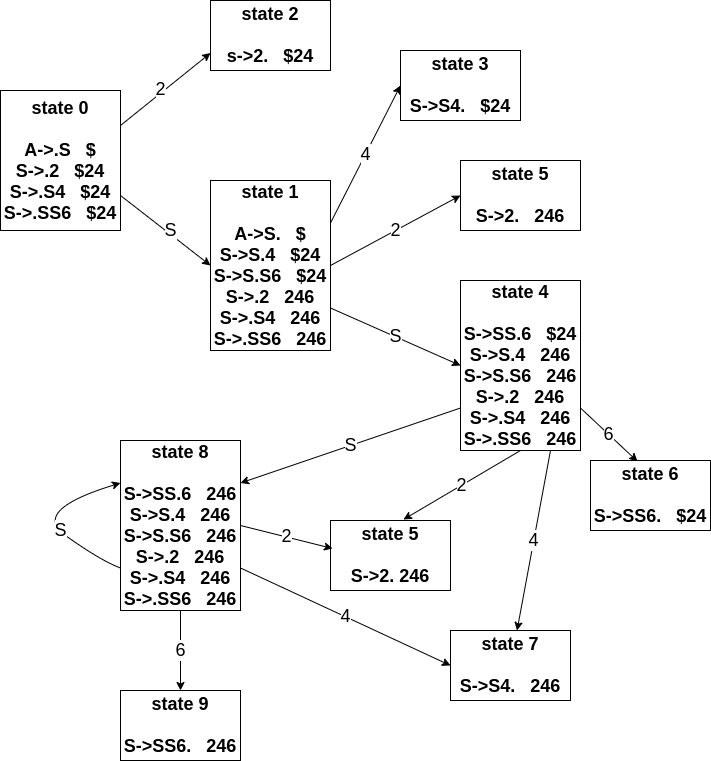
\includegraphics[scale=0.65]{compiler_hw2_q8.png}
\end{center}
ب) عکس جدول در زیر قرار داده شده است:
\begin{center}
	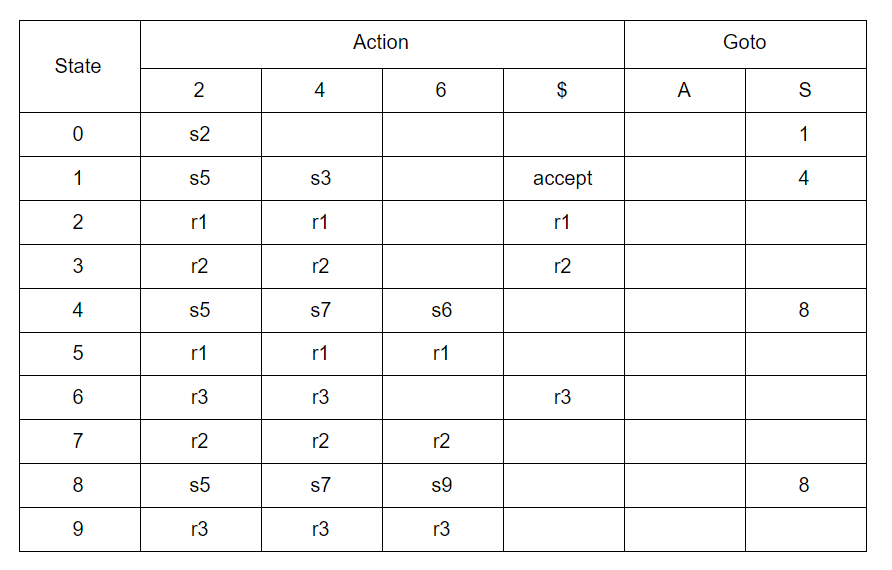
\includegraphics[scale=0.9]{compiler_hw2_q8_table.png}
\end{center}
ج) مراحل ایجاد درخت پارس $226422466$ را در پایین نوشته‌ایم: (دقت شود که حروفی که بین دو | می‌آیند در مرحله بعدی قرار است با هم، به کمک قاعده تولید reduce شوند)
\begin{latin}
	2
	\\
	|2|
	\\
	S
	\\
	S 2
	\\
	S |2|
	\\
	S S
	\\
	S S 6
	\\
	|S S 6|
	\\
	S
	\\
	S 4
	\\
	|S 4|
	\\
	S
	\\
	S 2
	\\
	S |2|
	\\
	S S
	\\
	S S 2
	\\
	S S |2|
	\\
	S S S
	\\
	S S S 4
	\\
	S S |S 4|
	\\
	S S S
	\\
	S S S 6
	\\
	S |S S 6|
	\\
	S S
	\\
	S S 6
	\\
	|S S 6|
	\\
	S
\end{latin}
در نهایت درخت پارس رشته به صورت زیر می‌شود: (به دو صورت عکس و کتابخانه خود latex نمایش داده شده است)
\begin{center}
	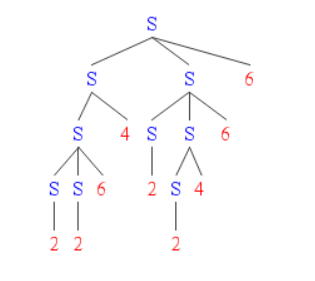
\includegraphics{226422466.png}
\end{center}

\begin {center}
\begin {tikzpicture}[-latex ,auto ,node distance =2 cm and 1cm ,on grid ,
semithick ,
state/.style ={ circle ,top color =white , bottom color = white ,
	draw,white , text=black , minimum width =1 cm}]
\node[state] (0){$S$};
\node[state] (1) [below left=of 0] {$S$};
\node[state] (2) [below =of 0] {$S$};
\node[state] (3) [below right=of 0] {\lr{6}};
\node[state] (4) [below left =of 1] {S};
\node[state] (5) [below =of 1] {\lr{4}};
\node[state] (6) [below =of 2] {$S$};
\node[state] (7) [below right=of 2] {\lr{$S$}};
\node[state] (8) [right =of 7] {\lr{6}};
\node[state] (9) [below left =of 4] {\lr{$S$}};
\node[state] (10) [below =of 4] {\lr{$S$}};
\node[state] (11) [below right=of 4] {\lr{6}};
\node[state] (12) [below =of 6] {\lr{2}};
\node[state] (13) [below =of 7] {\lr{$S$}};
\node[state] (14) [below right=of 7] {\lr{4}};
\node[state] (15) [below =of 9] {\lr{2}};
\node[state] (16) [below =of 10] {\lr{2}};
\node[state] (17) [below =of 13] {\lr{2}};


\path (0) edge [] node[left] {} (1);
\path (0) edge [] node[] {} (2);
\path (0) edge [] node[] {} (3);
\path (1) edge [] node[] {} (4);
\path (1) edge [] node[] {} (5);
\path (2) edge [] node[] {} (6);
\path (2) edge [] node[] {} (7);
\path (2) edge [] node[] {} (8);
\path (4) edge [] node[] {} (9);
\path (4) edge [] node[] {} (10);
\path (4) edge [] node[] {} (11);
\path (6) edge [] node[] {} (12);
\path (7) edge [] node[] {} (13);
\path (7) edge [] node[] {} (14);
\path (9) edge [] node[] {} (15);
\path (10) edge [] node[] {} (16);
\path (13) edge [] node[] {} (17);

\end{tikzpicture}
\end{center}

